
\chapter{Alternative cycles}
\section{Low temperature combustion}
\subsection{Homogeneous Charge Compression Ignition}
	The HCCI mode combines the principles of the homogeneous charge of the SI engine combined with the auto-ignition of the CI engine. The objective was to better control 2 strokes gasoline for weak mixture. They arrived to lower the consumption of 29\% (Honda Activated Radicals Combustion). The results pushed to make research for the 4-strokes. The main difference with SI engine is that the combustion don't occur with the waiting of flame propagation but the mixture ignite a bit everywhere. \\
	
	HCCI combines the advantages of diesel and gasoline engines. For example, it can burn any fuel and the NOx emission is reduced consequently. Indeed, since the fuel dilution is higher, the thermal efficiency is higher and thus NOx lower. Additionally, there is no rich zone and this decreases the soot.  The drawbacks are that the NO and HC emissions are increased, the load/speed range is is limited and no direct control. 
	
\subsubsection{Increasing working region}	
	\wrapfig{7}{l}{4}{0.3}{ch8/1}{ch8/1}	
	There are two main limits for HCCI. The lower limits is due to instability of the auto-ignition, illustrated by the Coefficient of Variation (CoV). The upper limit is described by the high energy release rate which lead to “knocking”. For what concerns the controllability, in traditional engines we have the injection and the spark, here not. In HCCI the auto ignition is function of many parameters having influence on the combustion. 	
	
	\paragraph{Variable compression ratio} The compression ratio is directly linked to the temperature at TDC. So if we can control it, we're done with the auto-ignition. But this is very complex. 
	
	\paragraph{Variable valve timing}
	This is already very often used on traditional engines, it allows to control the compression ratio through opening and closing of valves. 
	
	\wrapfig{3}{r}{3}{0.3}{ch8/2}{ch8/2}	
	\paragraph{Charge heating, turbocharging, injection timing, fuel mixture}
	Charge pre-heating is also an option but generally presents a certain inertia which limits to control for each cycle. Injection timing is used in alternative low temperature combustion (see below). Turbocharging and control of the inlet pressure is also an effective way of changing the combustion timing. For the mixture, we introduce a new number to characterize combustion in HCCI which is \textbf{CAI number (CAN)}. This is illustrated on the figure. We can use the different technologies together but the challenge lies in the transition from one mode to another.
	
	\paragraph{Current research} Consult the slides for more info but I don't think it is important. Be aware that Reactivity controlled Compression Ignition is experimented, we use small gasoline quantity in diesel. This method lowers the soot and NOx emission compared to full diesel. 

\section{Other cycles}
\paragraph{Atkinson cycle}
	\minifig{ch8/3}{ch8/4}{0.3}{0.3}{0.3}{0.3}
	The Atkinson cycle is an Otto cycle but with different compression and expansion ratio. Indeed, in Otto cycle, the compression and expansion ratio are the same, but this let a still high pressure at the end of expansion. The Atkinson idea is to take advantage of this last pressure. This would provide indeed more efficiency but this is complex. This is achieved by opening the exhaust later, but then power density decreases (we can compensate by supercharger $\rightarrow$ Miller), used in hybrid cars (electric for high loads). 

\paragraph{Scuderi cycle} The idea is to have to combustion chamber, the first one exhaust goes into the other for a second combustion. 

\begin{center}
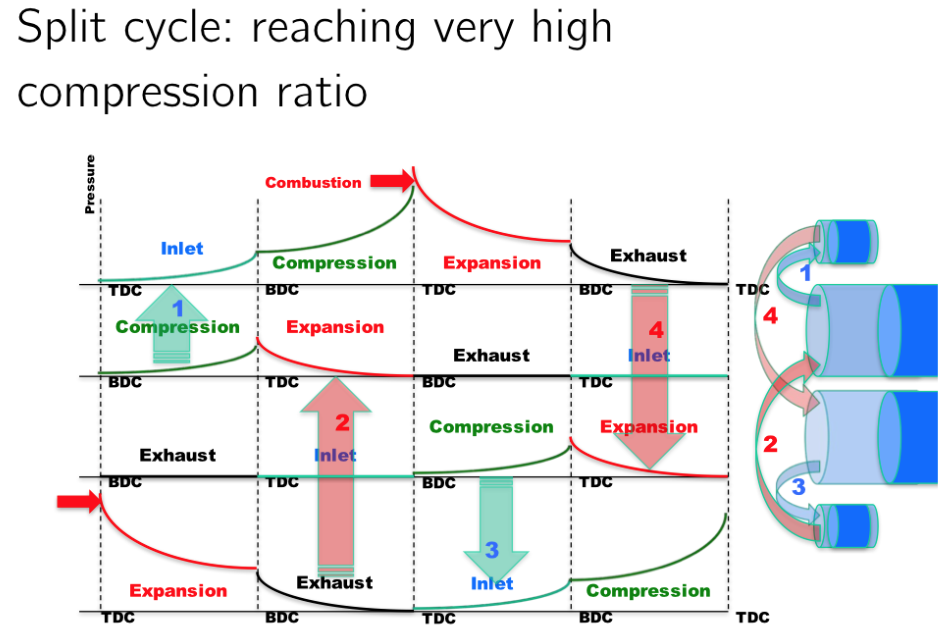
\includegraphics[scale=0.5]{ch8/5}
\end{center}

\textbf{End of the story, enjoy!}